\documentclass[12pt,openright,oneside,a4paper,chapter=TITLE,english,french,spanish,brazil,sumario=abnt-6027-2012]{abntex2}
\DisemulatePackage{setspace}
\usepackage{setspace}
\usepackage{textcomp}
\usepackage{gensymb}
\DeclareUnicodeCharacter{00B0}{\degree}
\usepackage{lmodern}
\usepackage[T1]{fontenc}
\usepackage[utf8]{inputenc}
\usepackage{indentfirst}
\usepackage[dvipsnames]{xcolor}
\usepackage{graphicx}
\graphicspath{{figuras/}{graficos/}}
\usepackage{microtype}
\usepackage{enumitem}
% !TeX root = ../tese_modelo.tex
\newcommand{\citar}{\textcolor{red}{[CITAR]}}
\newcommand{\preencher}[1]{\textcolor{red}{\textbf{[A PREENCHER:} \textit{#1}\textbf{]}}}
% \novo{}: texto recém-inserido (revisão). Aprovar = trocar \textcolor{red}{#1} por #1.
\newcommand{\novo}[1]{\textcolor{red}{#1}}
% \aref{ap:...} -> "Apêndice N" com hyperlink (corrige o \autoref em apêndices).
\newcommand{\aref}[1]{{\def\chapterautorefname{Apêndice}\autoref{#1}}}
% \verde{}: incorporações da revisão crítica. Aprovar = trocar por #1.
\newcommand{\verde}[1]{\textcolor{ForestGreen}{#1}}
% \magenta{}: citações sugeridas, a avaliar.
\newcommand{\magenta}[1]{\textcolor{magenta}{#1}}

\usepackage[alf,bibjustif,abnt-etal-text=it,abnt-etal-list=2,abnt-etal-cite=2]{abntex2cite}
\usepackage{multicol}
\usepackage{verbatim}
\usepackage{listings}
\lstset{basicstyle=\ttfamily\footnotesize,breaklines=true,breakindent=0pt,
        columns=fullflexible,keepspaces=true,frame=single,framerule=0.3pt,
        showstringspaces=false,xleftmargin=6pt,xrightmargin=6pt,breakautoindent=false}
\usepackage{imakeidx}
\usepackage{nomencl}
\makenomenclature
\usepackage{isotope}
\counterwithin{figure}{chapter}
\counterwithin{table}{chapter}
\usepackage{amsmath}
\usepackage{amssymb}
\usepackage{booktabs}
\usepackage{tikz}
\usepackage{array}
\usepackage{longtable}
\usepackage{multirow}
\usepackage{subcaption}
\usepackage{tocloft}
\usepackage{pdfpages}

% Colunas centralizadas de largura fixa (padrão de tabelas)
\newcolumntype{P}[1]{>{\centering\arraybackslash}p{#1}}
\newcolumntype{M}[1]{>{\centering\arraybackslash}m{#1}}

% ---------------------------------------------------------------
% DADOS DE IDENTIFICAÇÃO (capa e folha de rosto) --- PREENCHER
% ---------------------------------------------------------------
\titulo{[TÍTULO DO TRABALHO]}
\autor{[NOME COMPLETO DO AUTOR]}
\local{[CIDADE]}
\data{[ANO]}
\orientador{[Titulação e nome do orientador]}
\coorientador{[Titulação e nome do coorientador, se houver]}
\instituicao{%
	[UNIVERSIDADE]
	\par
	[UNIDADE ACADÊMICA]
	\par
	[DEPARTAMENTO]}
\tipotrabalho{[Tese (Doutorado) / Dissertação (Mestrado)]}
\preambulo{[Natureza do trabalho, programa de pós-graduação, departamento e instituição, e objetivo (por exemplo, requisito parcial para a obtenção do título de ...).]}

\definecolor{blue}{RGB}{41,5,195}
\makeatletter
\hypersetup{
	pdftitle={\@title}, pdfauthor={\@author}, pdfsubject={\imprimirpreambulo},
	pdfcreator={LaTeX with abnTeX2},
	pdfkeywords={[palavra-chave 1], [palavra-chave 2], [palavra-chave 3]},
	colorlinks=true, linkcolor=blue, citecolor=blue, filecolor=magenta, urlcolor=blue,
	bookmarksdepth=4
}
\setlength{\@fptop}{5pt}
\makeatother

% Quadros e lista de quadros
\newcommand{\quadroname}{Quadro}
\newcommand{\listofquadrosname}{Lista de quadros}
\newfloat[chapter]{quadro}{loq}{\quadroname}
\newlistof{listofquadros}{loq}{\listofquadrosname}
\newlistentry{quadro}{loq}{0}
\setfloatadjustment{quadro}{\centering}
\counterwithout{quadro}{chapter}
\renewcommand{\cftquadroname}{\quadroname\space}
\renewcommand*{\cftquadroaftersnum}{\hfill--\hfill}
\setfloatlocations{quadro}{hbtp}

% Espaçamentos e títulos
\setlength{\parindent}{1.3cm}
\setlength{\parskip}{0.2cm}
\renewcommand{\ABNTEXchapterfont}{\fontfamily{lmr}\fontseries{b}\selectfont}
\renewcommand{\ABNTEXsectionfont}{\fontfamily{lmr}\fontseries{b}\selectfont}
\renewcommand{\chaptitlefont}{\normalfont\large\bfseries}
\renewcommand{\cftsectionfont}{\bfseries}
\renewcommand{\cftsubsectionfont}{\normalfont}
\renewcommand{\cftsubsubsectionfont}{\normalfont}
\renewcommand{\cftparagraphfont}{\normalfont}
\renewcommand{\ABNTEXsectionfontsize}{\normalsize}
\renewcommand{\ABNTEXsubsectionfontsize}{\normalsize}
\renewcommand{\cftpartfont}{\cftchapterfont}
\renewcommand{\cftpartpagefont}{\cftchapterpagefont}
\renewcommand{\printparttitle}[1]{\parttitlefont\MakeTextUppercase{#1}}

\makeindex

\begin{document}
	\setlength{\abovedisplayskip}{5pt}
	\setlength{\abovedisplayshortskip}{0pt}
	\setlength{\belowdisplayskip}{12pt}
	\setlength{\belowdisplayshortskip}{12pt}
	\setlength{\afterchapskip}{18pt}

	\selectlanguage{brazil}
	\frenchspacing

	% --- Pré-textuais ---
	% !TeX root = ../tese_modelo.tex
\imprimircapa

	% !TeX root = ../tese_modelo.tex
\imprimirfolhaderosto*
\newpage

	% !TeX root = ../tese_modelo.tex
% Resumo (português) e Abstract (inglês)

\setlength{\absparsep}{18pt}
\begin{resumo}

\noindent [Texto do resumo em um único parágrafo, justificado.]

\vspace{\onelineskip}

\noindent
\textbf{Palavras-chave}: [Palavra 1]; [Palavra 2]; [Palavra 3].
\end{resumo}

\begin{resumo}[Abstract]
\begin{otherlanguage*}{english}

	\noindent [Abstract text in a single paragraph.]

	\vspace{\onelineskip}

	\noindent
	\textbf{Keywords}: [Word 1]; [Word 2]; [Word 3].
\end{otherlanguage*}
\end{resumo}

	% !TeX root = ../tese_modelo.tex
\begin{resumo}[Abstract]
	\begin{otherlanguage*}{english}
		[Abstract text in a single paragraph.]

		\textbf{Keywords}: [Word 1]. [Word 2]. [Word 3].
	\end{otherlanguage*}
\end{resumo}

	% !TeX root = ../tese_modelo.tex
\pdfbookmark[0]{\listfigurename}{lof}
\listoffigures*
\cleardoublepage

\pdfbookmark[0]{\listtablename}{lot}
\listoftables*
\cleardoublepage

% Siglas: ordem alfabética; inglês em itálico com tradução entre parênteses
\begin{siglas}
	\item[ABNT] Associação Brasileira de Normas Técnicas
	\item[{[SIGLA]}] \textit{[Forma por extenso em inglês]} ([tradução])
\end{siglas}

% Símbolos: latinos primeiro, depois gregos, cada grupo em ordem alfabética
\begin{simbolos}
	\item[$x$] [Descrição do símbolo latino]
	\item[$\alpha$] [Descrição do símbolo grego]
\end{simbolos}

\pdfbookmark[0]{\contentsname}{toc}
\tableofcontents*
\cleardoublepage


	% --- Textuais ---
	\textual
	\part{[Título da parte]}\label{part:um}
	% !TeX root = ../tese_modelo.tex
\chapter{[Título do Capítulo]}
\label{ch:modelo}

[Parágrafo de apresentação do capítulo: o que será tratado, por que importa para o trabalho e como o capítulo se organiza.] \cite{chave2024exemplo}.

\section{[Título da Seção]}
\label{sec:modelo_secao}

Texto corrido com valor numérico e unidade, como $1{,}5$~m de comprimento e $20$~kg de massa. Citação com autor na frase: conforme \citeonline{chave2024exemplo}. Referências cruzadas: \autoref{tab:modelo}, \autoref{fig:modelo}, \autoref{eq:modelo} e \aref{ap:modelo}.

\begin{equation}
	y = a\,x + b,
	\label{eq:modelo}
\end{equation}
onde $y$ é a variável dependente, $x$ a variável independente, $a$ o coeficiente angular e $b$ o coeficiente linear.

\begin{table}[h!]\centering
	\setlength{\tabcolsep}{8pt}
	\renewcommand{\arraystretch}{1.2}
	\caption[Título curto da tabela]{Legenda completa da tabela. Elaborado pelo autor.}\label{tab:modelo}
	\small
	\begin{tabular}{M{2,4cm}M{4,2cm}M{2,4cm}}\toprule
		\textbf{Coluna A} & \textbf{Coluna B} & \textbf{Coluna C} \\
		\midrule
		$1{,}0$ & texto & $2{,}5$~kg \\
		\bottomrule
	\end{tabular}
\end{table}

\begin{figure}[h!]
	\centering
	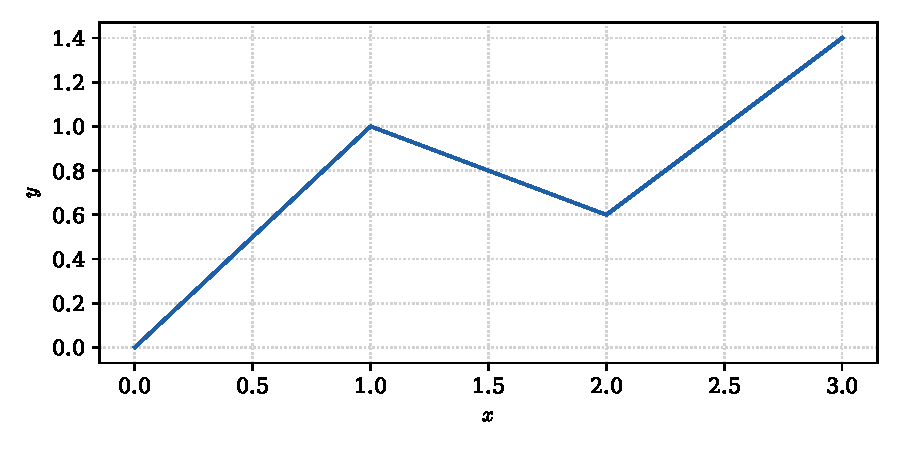
\includegraphics[width=0.95\linewidth]{figuras/exemplo.pdf}
	\caption[Título curto da figura]{Legenda completa da figura. Elaborado pelo autor.}
	\label{fig:modelo}
\end{figure}

\begin{figure}[h!]
	\centering
	\begin{subfigure}[b]{0.49\linewidth}\centering
		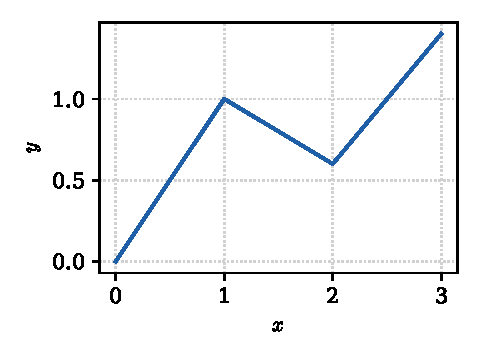
\includegraphics[width=\linewidth]{figuras/exemplo_a.pdf}
		\caption{Painel A}\end{subfigure}\hfill
	\begin{subfigure}[b]{0.49\linewidth}\centering
		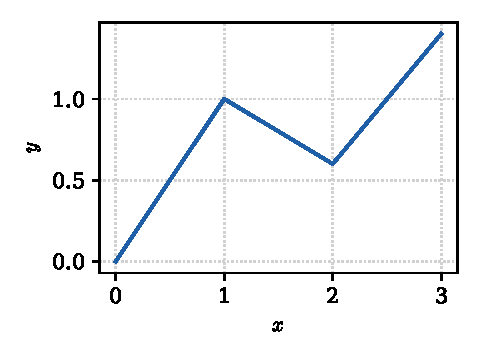
\includegraphics[width=\linewidth]{figuras/exemplo_b.pdf}
		\caption{Painel B}\end{subfigure}
	\caption[Título curto das subfiguras]{Legenda geral das subfiguras. Elaborado pelo autor.}
	\label{fig:modelo_sub}
\end{figure}

\section{\novo{[Seção com Texto Novo]}}
\label{sec:modelo_novo}

\novo{Texto recém-inserido, em vermelho até a aprovação.} \preencher{informação pendente}


	% --- Pós-textuais ---
	\postextual
	\bibliography{referencias}

	\begin{apendicesenv}
	\partapendices
	% !TeX root = ../tese_modelo.tex
\chapter{[Título do Apêndice]}
\label{ap:modelo}

[Texto do apêndice.] Listagens de código ou inputs:

\begin{lstlisting}
exemplo de listagem
\end{lstlisting}

	\end{apendicesenv}

	\printindex
\end{document}
